\section{Teilaufgabe C)}
\textbf{Versuchen Sie, die Laufzeit Ihres Programms zu beschleunigen! Dokumentieren Sie
einzelne Verbesserungsideen und die jeweiligen Laufzeitveränderungen für eine lokale
Ausführung Ihres Programms bei der Erzeugung einer 10-tps-Datenbank!}

\subsection{Transaction}
Um den Durchsatz der Daten zu erhöhen lassen sich die Queries in einer
Transaction zusammenfassen.  

Dazu muss die Option \textit{autoCommit} abgeschaltet werden und die Transaktion
mit einem manuellen \textit{commit} zum Server geschickt werden. Wir müssen also
unseren \nameref{lst:tpsv1} erweitern. Dafür legen wir 2 neue Funktionen an und
erweitern nebenbei die anderen Funktionen um ein zuschaltbares Debug-Logging.

\begin{lstlisting}
	public void beginTransaktion() {
		try {
			connection.databaseLink.setAutoCommit(false);
		} catch (SQLException e) {
			e.printStackTrace();
		}
	}
	
	public void endAndCommitTransaction() {
		try {
			connection.databaseLink.commit();
			connection.databaseLink.setAutoCommit(true);
		} catch (SQLException e) {
			e.printStackTrace();
		}
	}
\end{lstlisting}


Jetzt brauchen wir noch die funktionalität, um die Funktionen zu benutzen. Damit
wir recht flexibel sind implentieren wir hierfür ein Konsolen-Menü. Dieses
erstellt uns dann eine Benchmark Klasse die die tpsCreator-Klasse alle nötigen
Parameter übergibt und das Benchmarking ausführt.\\

\begin{lstlisting}

	public static int renderMenu() {
		System.out.println("======================- Benchmark Menu -===========================");
		System.out.println("= Wähle bitte eine der folgende Optionen:                         =");
		System.out.println("= (1) Benchmark, Debug Log, incl. drop & create                   =");
		System.out.println("= (2) Benchmark, Debug Log, excl. drop & create                   =");
		System.out.println("= (3) Benchmark, Debug Log, transactions, incl. drop & create     =");
		System.out.println("= (4) Benchmark, Debug Log, transactions, excl. drop & create     =");
		System.out.println("= (5) Benchmark, incl. drop & create                              =");
		System.out.println("= (6) Benchmark, excl. drop & create                              =");
		System.out.println("= (7) Benchmark, transactions, incl. drop & create                =");
		System.out.println("= (8) Benchmark, transactions, excl. drop & create                =");
		System.out.println("===================================================================");
		System.out.print("= Auswahl: ");
		
		return ConsoleReader.readInt();
	}
\end{lstlisting}

 
Die Queries, die mittels einer Transaktion übertragen worden sind, sind bei
einer 1-tps-Datenbank um \ca das 11fache schneller als die Queries die einzelnt
zum Server geschcikt worden sind.

\begin{figure}[!htbp] 
    \subfigure[mit
    Transactions]{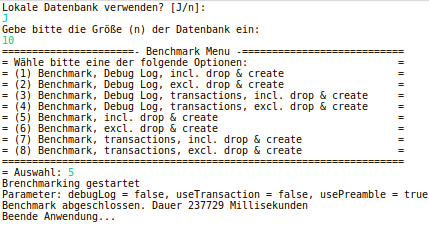
\includegraphics[width=0.49\textwidth]{Bilder/Auswahl_014.png}}
    \subfigure[ohne
    Transaction]{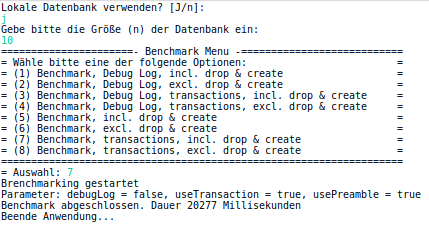
\includegraphics[width=0.49\textwidth]{Bilder/Auswahl_015.png}}
\end{figure} 


\subsection{Prepared Statements}
Selbst in einer Transaktion wird jeder einzelne Query validiert. Wir besitzen
nun aber eine Masse von gleich strukturierten Statements. Jeden einzelnen zu
validieren kostet den Server Zeit und Ressourcen.
 
 Wir suchen also eine Möglichkeit eine vorher definierte und validierte Struktur
 eines Queries zu bekommen. Dazu bietet sich das \textbf{Prepared Statement} an.
 Wie der Name schon sagt, wird dieser Query einmal zum Server geschickt und
 validiert. Anschließend kann man mit der Reference des Prepared Statements
 schnell und sicher die Daten dem Server übergeben.
 
Die umgeschriebene Funktion für Accounts sieht nun folgendermaßen aus:
 \begin{lstlisting}

	public boolean createAccountTupel(int n) {
		int localConst = n*10000;
		int localRandom;		
		try {
			PreparedStatement insertBranches = connection.databaseLink.prepareStatement("INSERT INTO accounts (accid, NAME, balance, address, branchid) VALUES(?, 'account', 0,'test', ?)");
			
			for (int i = 1; i <= localConst; i++) {
				localRandom = ThreadLocalRandom.current().nextInt(1, n + 1);
				insertBranches.setInt(1, i);
				insertBranches.setInt(2, localRandom);
				insertBranches.addBatch();
				
				if(isDebug) {
					System.out.println("INSERT INTO branches (branchid, branchname, balance,address) VALUES(" + i + ", 'branch', 0, 'branch')");
				}
			}

			insertBranches.executeBatch();
			return true;
		} catch (SQLException e) {
			e.printStackTrace();
		}
		return false;
	}
 \end{lstlisting}

Eine gute Eigenschaft von den Prepared Statements ist, dass sie die
Transaktionsverwaltung schon intregriert haben und damit bei gleichen Queries
deutlich schneller sind als ein normales Statement, welches ein und den selben
Query immer und immer wieder ausführt. Diese Eigenschaft besitzt ein
Prepared Statement auch, wenn das Feature \textit{autoCommit} aktiviert ist.

Um aber aussagekräftige Benchmarks zu erhalten, ist gerade das Feature
hinderlich, Wir möchten ja die Queries auch ohne Transaktion ausführen können,
deshalb müssen wir uns eine alte Kopie der Klasse behalten und bei Bedarf
instanziieren.
\begin{center}
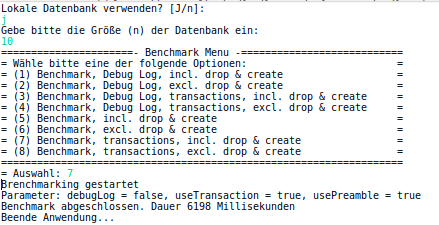
\includegraphics[scale=0.8]{Bilder/Auswahl_016.png}
\end{center}
Mit den Prepared Statement ist unser Benchmark jetzt \textbf{36fach} schneller
als unser ursprüngliches Benchmark Tool.

\subsection{IDs vom Server generieren lassen}
Momentan benutzen wir die Ressourcen von unserem Javaprogramm. Da wir aber so
viel wie Möglich vom Server verarbeiten lassen wollen, lagern wir das Generieren
der Branchen-IDs auf unseren Server aus, denn dieser hat mit Sicherheit die
Möglichkeit aus unserem SQL-Query etwas Effizentes zu generieren.

Wir müssen uns also den Zufallszahlengenerator von PostgreSQL benutzen um uns
eine ID zu genrieren.

\begin{lstlisting}[language=sql]
SELECT rand();
\end{lstlisting}

Diese Funktion liefert uns eine Gleitkommazahl zwischen 0 und 1. Diese Zahl
müssen wir anschließend nur noch $ \cdot  n + 1 $ rechnen um eine zufällige ID
zwischen 1 und $n$ zu erzeugen. Das am Ende stehende $ + 1$ soll dafür sorgen,
dass $n$ auch generiert werden kann. Anschließend schneiden wir mittels \textit{trunc} noch
die Kommastellen ab.

Unser Query, der uns die IDs generiert, sieht dann folgendermaßen aus:
\begin{lstlisting}[language=sql]
SELECT trunc(random() *  n  + 1);
\end{lstlisting}

Diesen Query können wir jetzt auf unser Prepared Statement anwenden:
\begin{lstlisting}[language=sql]
INSERT INTO accounts (accid, NAME, balance, address, branchid) VALUES(?, 'account', 0,'test', trunc(random() * n + 1))
\end{lstlisting}

Diese Optimierung spart uns bei einer  \textbf{10-tps-Datenbank} nochmal \ca
500 Millisekunden. Jedoch ist es jetzt nicht mehr Möglich im DebugLog die
generierte ID zu überprüfen.


\subsection{Adressauflösung von Domainnamen}
Um das Ergebnis noch mehr zu verbessern kommt jetzt das Feintuning. Dazu
schauen wir uns jetzt nicht das DBMS an, sondern DNS-Server.

Hier besteht ein massiver Nachteil gegenüber der herkömmlicher IP. Jeder
DNS-Server \bzw DNS-Cache muss in irgendeiner Tabelle nachschauen, welche Domain
zu welcher IP gehört. 

Selbst der lokale DNS-Cache muss dies \zB für \textbf{localhost} machen.
Zugriffe bedeuten bekanntlich Zeit. Möchten wir also diese Zugriffszeiten
umgehen, brauchen wir einfach nur die IP-Adresse statt des Domainnamens
einzugeben. Dies wäre für \textbf{localhost} entweder \gqq{127.0.0.1} als
IPv4-Schreibweiße oder \gqq{[::1]} als IPv6 Schreibweise.

-- bis hierher bin ich gekommen .- lg mario
ps: habe nicht auf rächtschreibung geachtet, habe einfach mal drauf los getippz,
vieles ist noch überarbeitungswürdig. Es muss noch das Optimierte Programm in
den Anhang. An einigen Stellen mittels nameref darauf verwiesen werden und
eindeutig sollte der gesamte Text mal durch word geschickt werden.
\clearpage